%%%%%%%%%%%%%%%%%%%%%%%%%%%%%%%%%%%%%%
%
% This is how you write code:
%
% \begin{minted}{matlab}
% foo = [2 1 0;1 4 3;2 4.5 6];
% \end{minted}
%

% This is how you import code:
% 
% \inputminted[linenos]{matlab}{foo_bar.m}
%
 
% Most figures are imported this way:
%
% \begin{figure}
% \includegraphics[width=\textwidth]{foo_figure}
% \caption{This is a caption}
% \end{figure}

% This is a matrix:
%
% \begin{equation}
% H =
%  \left[
%  \begin{matrix}
%    1 & 2 &  3 &  4 \\ 
%    5 & 6 &  7 &  8 \\ 
%    0 & 9 & 10 & 11 \\ 
%    0 & 0 & 12 &  0
%  \end{matrix} 
% \right]
%\end{equation}
%
%%%%%%%%%%%%%%%%%%%%%%%%%%%%%%%%%%%%%%

% For better looking tables
\newcommand{\head}[1]{\textnormal{\textbf{#1}}}

\documentclass[00-main.tex]{subfiles}
\begin{document}


\section*{Problem Two}

In the following $X_n$ is the number of individuals in the $n$'th generation,
 $X_0$ is the initial population, $\mu = E[$\textit{children per individual}$]$, $p_j = P\{$\textit{an individual has }$j$\textit{ offspring}$\}$. The distributions that are analyzed are listed in \cref{p-values}
 
\begin{table}[!htbp]
\centering
\begin{tabular}{ccccc}
  \hline
  \noalign{\smallskip}
  \head{ } & \head{$p_0$} & \head{$p_1$} & \head{$p_2$} & \head{$p_3$}\\
  \hline
  \noalign{\smallskip}
  \textbf{I} & 0.6 & 0.05 & 0.15 & 0.2 \\
  \textbf{II} & 0.25 & 0.60 & 0.10 & 0.05 \\
  \hline
\end{tabular}
\caption{The probability distributions given in Problem Two.}
\label{p-values}
\end{table}

Chapter 4.7 in \cite{ross} presents some results that are used in this problem. Below is some properties of branching processes discussed.

Generally, the mean number, and the variance, of offspring of a single individual is

\begin{equation}
\label{meanvar}
\mu = \sum_{j=0}^{\infty} jP_j \quad \quad \text{and} \quad \quad \sigma^2 = \sum_{j=0}^{\infty} (j-\mu)^2P_j
\end{equation}

respectively.

For both our distributions $\mu = 0.95$, and since $\mu < 1$ the population will eventually die out. Defining $Z_i$ to be the number of offspring of the $i$'th individual for the $(n-1)$th generation, one can find 

\begin{equation}
X_n = \sum_{i=1}^{X_{n-1}} Z_i
\end{equation}

in the edge case where $X_0=1$. One can then obtain

\begin{equation}
E[X_n] = E[E[X_n | X_{n-1}]] = E\left[ E\left[ \sum_{i=1}^{X_{n-1}} Z_i | X_{i-1} \right] \right] = E[X_{n-1}] \mu 
\end{equation}

which leads to the result

\begin{equation}
\label{mean}
E[X_1] = \mu, \quad E[X_2] = \mu E[X_1] = \mu^2, \quad \cdots, \quad E[X_n] = \mu^n.
\end{equation}

It can then be shown that the variance is

\begin{align}
\label{variance}
  Var(X_n) = \left\{ 
  \begin{array}{l l l}
     \sigma^2 \mu^{n-1} \cdot \frac{1-\mu^n}{1-\mu}, \quad &\mu \neq 1\\
     n \sigma^2, \quad  &\mu = 1 \\
  \end{array} \right.
\end{align}

When doing simulations, the estimated mean value and standard deviation is given by

\begin{equation}
\bar{X} = \frac{1}{n} \sum_{i=1}^{n} X_i, \qquad S^2 = \frac{1}{n-1}\sum_{i=1}^{n} X_i - \bar{X},
\end{equation}

respectively. 

\subsection*{a.}

The mean and standard deviation is found analytically from \cref{meanvar}, \cref{mean} and \cref{variance}, and is presented in \cref{anatable}.

\begin{table}[!htbp]
\centering
\begin{tabular}{ccccc}
  \hline
  \noalign{\smallskip}
  $n$ & $E[X_n]$ & $SD_I[X_n]$ & $SD_{II}[X_n]$   \\
  \hline
  \noalign{\smallskip}
  10   & 0.5987 & 2.7977 & 2.7692 &    \\
  100  & 0.0059 & 0.4379 & 0.0678 &    \\
  1000 & 5.2912e-23 & 4.1529e-11 & 2.4697e-11 &    \\
  \hline
\end{tabular}
\caption{Analytical values of the mean $E[X_n]$ and the standard deviation, SD ($=Var^{\frac{1}{2}}[X_n]$) for distribution I and II.}
\label{anatable}
\end{table}


The branching process was simulated a hundred thousand times for each of the probability distributions. The values in \cref{simtable} were computed by running

\begin{minted}{matlab}
% No. of simulations
N = 100000;
% Size of the first population
init = 1;
% Distribution I = p1 and II = p2
p1 = [0.60 0.05 0.15 0.20];
p2 = [0.25 0.60 0.10 0.05];
% Run the simulations for I and II
branchtrials(N, init, p1);
branchtrials(N, init, p2);
\end{minted}


\begin{table}[!htbp]
\centering
\begin{tabular}{ccccccc}
  \hline
  \noalign{\smallskip}
  $n$ & $E_I[X_n]$ &$E_{II}[X_n]$ &$E_{III}[X_n]$ & $SD_I[X_n]$ & $SD_{II}[X_n]$ & $SD_{III}[X_n]$   \\
  \hline
  \noalign{\smallskip}
  10   & 0.6007 & 0.5989 & 0.0554 & 2.8099 & 1.6708 & 0.4662 \\
  100  & 0.0060 & 0.0050 & 0      & 0.4583 & 0.2392 & 0      \\
  1000 & 0      & 0      & 0      & 0      & 0      & 0      \\
  \hline
\end{tabular}
\caption{Simulated values of the mean $E[X_n]$ and the standard deviation, SD ($=Var^{\frac{1}{2}}[X_n]$) for distribution I and II.}
\label{simtable}
\end{table}

The simulated values is indeed very close to the ones found analytically for both distributions. Given that the \textsc{matlab} rand()-function is uniform, the simulated values would probably become even more accurate if the number of simulations is increased. No simulation ever reached $n=1000$, but this is only natural considering the low probability for that to happen. 

Case (i), (ii) and (iii) are presented in \cref{simtable2} for both distributions.

\begin{table}[!htbp]
\centering
\begin{tabular}{ccccccc}
  \hline
  \noalign{\smallskip}
   & \multicolumn{2}{c|}{Distribution I} & \multicolumn{2}{c|}{Distribution II} & \multicolumn{2}{c}{Distribution III} \\
  \head{Case} & $E[\cdot]$ &$SD[\cdot]$ & $ E[\cdot]$ &$SD[\cdot]$ & $ E[\cdot]$ &$SD[\cdot]$ \\
  \hline
  \noalign{\smallskip}
  (i)    & 4.5197 & 7.1409    &    8.2460 & 10.8820   & 3.5185 & 2.5587\\
  (ii)   & 19.9991 & 109.4967 &    19.9830 & 65.9630  & 3.9787 & 7.0344\\
  (iii)  & 2.9699 & 5.4466    &    2.3411 & 2.9429    & 1.5572 & 1.1611\\
  \hline
\end{tabular}
\caption{Simulated values of the mean $E[X_n]$ and the standard deviation, SD ($=Var^{\frac{1}{2}}[X_n]$) for distribution I and II.}
\label{simtable2}
\end{table}

\subsection{b.}

\begin{minted}{matlab}
% Defining a third distribution
p3 = [0.50 0.30 0.15 0.05];
% Run the simulations for III
branchtrials(N, init, p3);
\end{minted}

\begin{figure}[!htbp]
  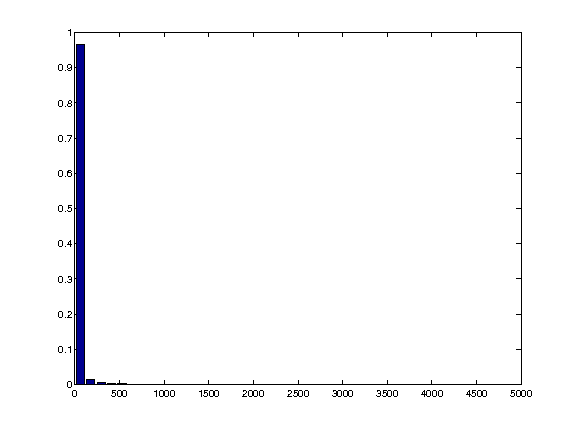
\includegraphics[width=\textwidth/2]{p1/gen.png}
  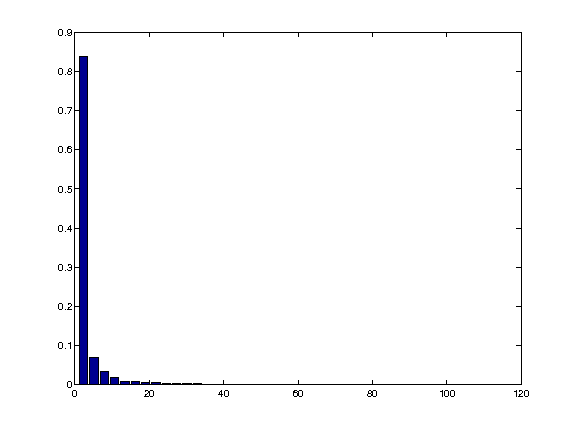
\includegraphics[width=\textwidth/2]{p1/pop.png}
  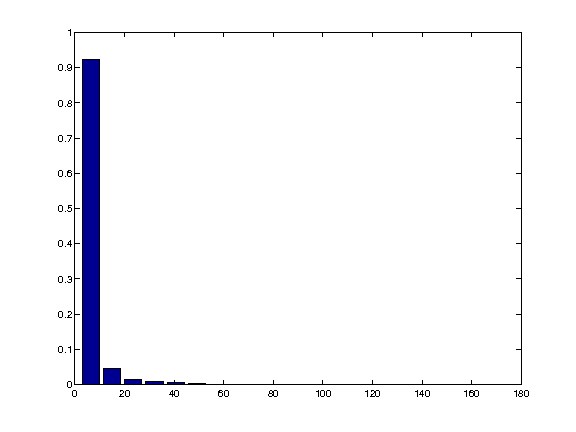
\includegraphics[width=\textwidth/1]{p1/largest.png}
  \caption{Case (i), (ii) and (iii) for distribution I}
  \label{I}
\end{figure}


\begin{figure}[!htbp]
  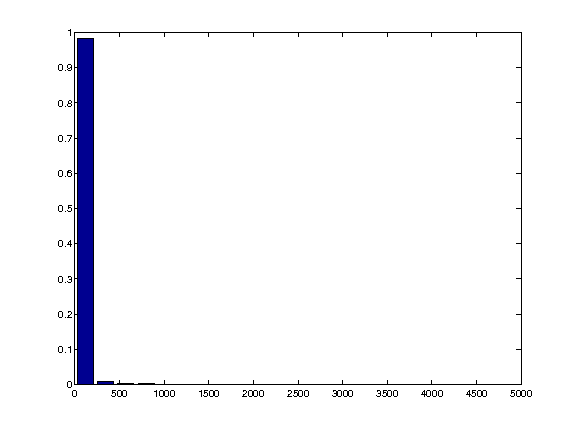
\includegraphics[width=\textwidth/2]{p2/gen.png}
    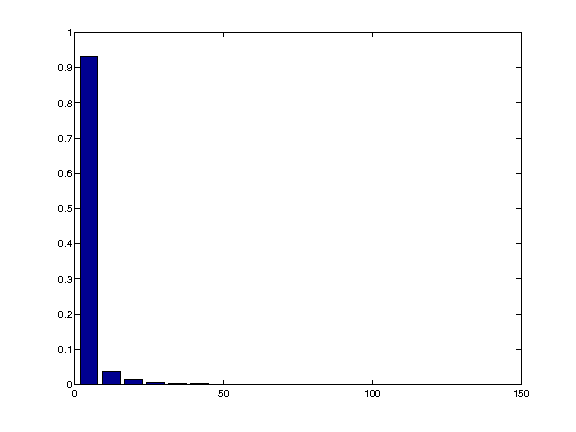
\includegraphics[width=\textwidth/2]{p2/pop.png}
  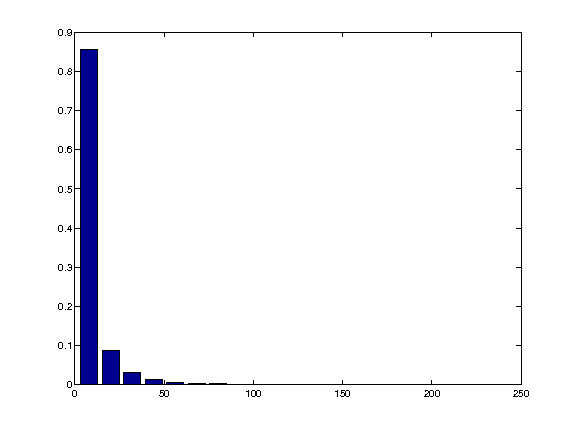
\includegraphics[width=\textwidth/1]{p2/largest.png}
  \caption{Case (i), (ii) and (iii) for distribution II}
  \label{II}
\end{figure}


\begin{figure}[!htbp]
  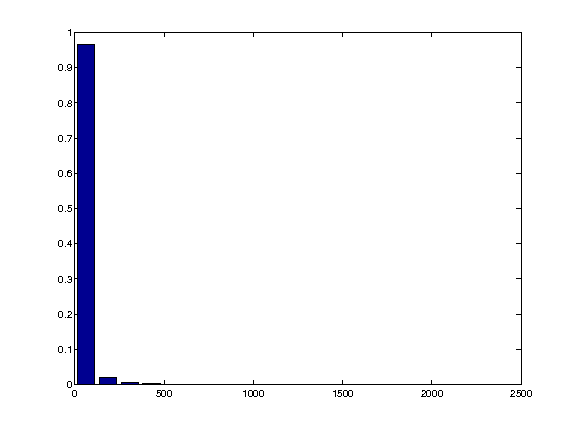
\includegraphics[width=\textwidth/2]{p3/gen.png}
    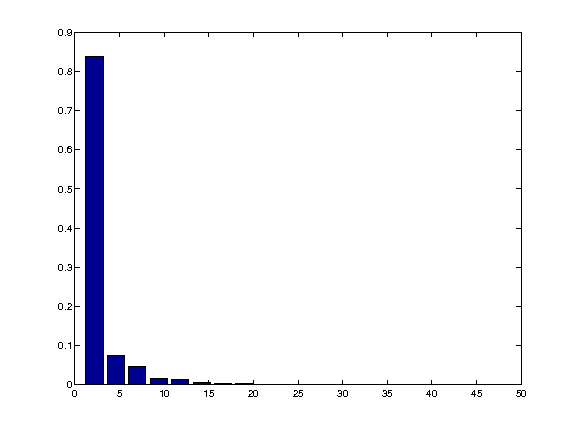
\includegraphics[width=\textwidth/2]{p3/pop.png}
  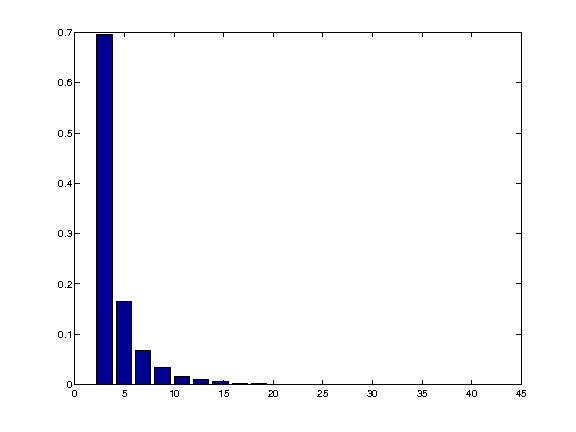
\includegraphics[width=\textwidth/1]{p3/largest.png}
  \caption{Case (i), (ii) and (iii) for distribution III}
  \label{III}
\end{figure}



\end{document}